\documentclass{article}
\usepackage{url}
\usepackage{hyperref}
\usepackage{tikz}
\usepackage{amsmath}
\usepackage{amssymb}
\usepackage[backend=biber]{biblatex}
\addbibresource{biblio.bib}

\newtheorem{theorem}{Theorem}
\newtheorem{definition}{Definition}

\title{INFO-F420 Project Report\\ Computing Smallest Convex Intersecting Polygon}
\author{Bataille Alex \\ Bouhdid Wassim}


\begin{document}
\maketitle 

\section{Introduction}
A natural generalization of convex hulls, a standard object in computation geometry, is to consider the smallest convex polygon 
that intersects all objects in a set $\mathcal{O}$. This is the problem considered and solved in \cite{Antoniadis_deBerg_Kisfaludi-Bak_Skarlatos_2025}, where the authors consider a smallest 
polygon to either have minimum-area, or minimum-perimeter. For the purpose of this project, we focused on the dynamic programming algorithm allowing to compute a minimum-perimeter polygon intersecting 
a set of segments in the plane (cf. Section 5 of \cite{Antoniadis_deBerg_Kisfaludi-Bak_Skarlatos_2025}). An \href{https://alexei-x.github.io/info-F420-project/}{interactive website} was developed to illustrate the main ideas of the algorithm. 

\section{The Exact Segment Problem}
We will thus consider a set $\mathcal{O}$ of $n$ segments in the plane. We want to compute a polygon $C_{opt}$ that has minimum-perimeter, intersecting all the segments (see Figure \ref{fig:segments-instance}). 
\begin{figure}[h] \centering 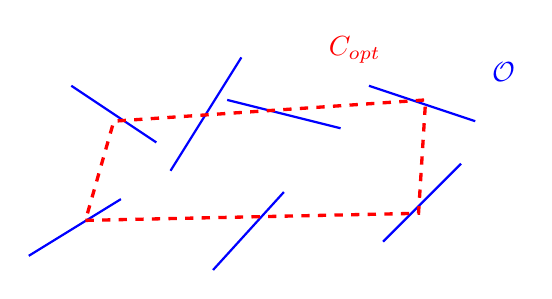
\begin{tikzpicture}[scale=0.9] 
    % Segments of O 
    \draw[thick, blue] (0.2,0.6) -- (1.5,1.4); 
    \draw[thick, blue] (0.8,3.0) -- (2.0,2.2); 
    \draw[thick, blue] (2.8,0.4) -- (3.8,1.5); 
    \draw[thick, blue] (3.0,2.8) -- (4.6,2.4); 
    \draw[thick, blue] (5.2,0.8) -- (6.3,1.9); 
    \draw[thick, blue] (5.0,3.0) -- (6.5,2.5); 
    \draw[thick, blue] (2.2,1.8) -- (3.2,3.4); 
    % A convex polygon intersecting all segments 
    \draw[dashed, red, very thick] (1.0,1.1)  -- (5.7,1.2) -- (5.8,2.8)  -- (1.4,2.5) -- cycle; 
    \node[blue] at (6.9,3.2) {$\mathcal O$}; 
    \node[red] at (4.8,3.5) {$C_{opt}$};
\end{tikzpicture} 
\caption{An instance of the Exact Segment Problem. The set $\mathcal O$ consists of line segments (blue). The dashed polygon $C_{opt}$ is a convex polygon intersecting every segment of $\mathcal O$.} 
    \label{fig:segments-instance} 
\end{figure}


We will use the same notations as \cite{Antoniadis_deBerg_Kisfaludi-Bak_Skarlatos_2025}, namely, let $C_{opt}$ denote the optimal solution, and $Y$ the set of all endpoints 
of the segments in $\mathcal{O}$. 


\section{The Subroutines and the TPP Reduction}

The algorithm uses two subroutines that reduce parts of the problem to the
Touring Polygons Problem (TPP).

\subsection{The Touring Polygons Problem}

\begin{definition}[Touring Polygons Problem]
Given a sequence of convex polygons $P_1, \ldots, P_k$, a start point $s$, and
an end point $t$, find the shortest path from $s$ to $t$ that visits $P_1, \ldots,
P_k$ in order (i.e., there exist points $q_i \in P_i$ appearing in index order
along the path).
\end{definition}

TPP was solved in \cite{10.1145/780542.780612} in $O(nk^2 \log n)$ time for
arbitrary convex polygons, and in $O(n^3 \log n)$ for segments and half-planes.

\subsection{The Reduction: Segments to Half-Planes}

The reduction works as follows. Fix two points $u, v$ on the $x$-axis and a set
$\mathcal{O}$ of $n$ segments. For each segment $o_i$, define its half-plane $H_i$
with respect to $u, v$.

We order the half-planes by sorting their outward normal vectors $\vec{n}_i$ in
clockwise order, starting from direction $(0, -1)$.
\begin{figure}[ht] 
    \centering 
    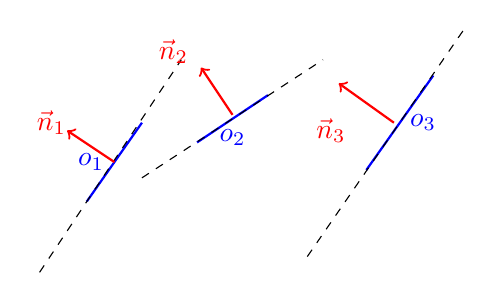
\begin{tikzpicture}[scale=1] 
    % segments 
    \draw[thick, blue] (0.8,1.2)--(1.5,2.2) node[midway,left] {$o_1$}; 
    \draw[thick, blue] (2.2,1.95)--(3.1,2.55) node[midway,below] {$o_2$}; 
    \draw[thick, blue] (4.35,1.6)--(5.2,2.8) node[midway,right] {$o_3$}; 
    % supporting lines 
    \draw[dashed] (0.2,0.3)--(2.0,3); 
    \draw[dashed] (1.5,1.5)--(3.8,3.0); 
    \draw[dashed] (3.6,0.5)--(5.6,3.4); 
    % normals 
    \draw[->,red,thick] (1.15,1.7)--(0.55,2.1); 
    \draw[->,red,thick] (2.65,2.3)--(2.25,2.9); 
    \draw[->,red,thick] (4.7,2.2)--(4.0,2.7); 
    \node[red] at (0.35,2.2) {$\vec n_1$}; 
    \node[red] at (1.9,3.1) {$\vec n_2$}; 
    \node[red] at (3.9,2.1) {$\vec n_3$}; 
\end{tikzpicture} 
    \caption{ Each segment $o_i$ defines a half-plane $H_i$. The half-planes are ordered according to the clockwise order of their outward normal vectors. } 
    \label{fig:halfplane-ordering} 
\end{figure}

This ordering is correct (Lemma 22) because any clockwise-oriented convex
chain $\Gamma$ from $u$ to $v$ in the upper half-plane that visits all $H_i$
must visit them in this prescribed order. The proof uses a queue-based
procedure: as $\Gamma$ exits half-planes, the exit points define visit points
$t_i \in H_i$ in index order. Convexity ensures that a half-plane with a
"later" normal cannot be exited before one with an "earlier" normal.
\begin{figure}[ht] \centering 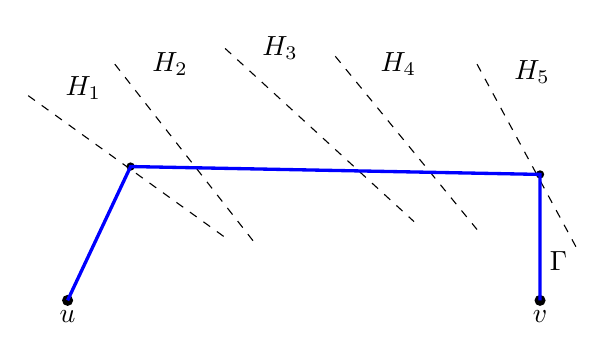
\begin{tikzpicture}[scale=1] 
    % u,v 
    \fill (0,0) circle (2pt) node[below] {$u$}; 
    \fill (6,0) circle (2pt) node[below] {$v$}; 
    % half-plane boundaries 
    \draw[dashed] (-0.5,2.6)--(2.0,0.8); 
    \draw[dashed] (0.6,3.0)--(2.4,0.7); 
    \draw[dashed] (2.0,3.2)--(4.4,1.0); 
    \draw[dashed] (3.4,3.1)--(5.2,0.9); 
    \draw[dashed] (5.2,3.0)--(6.5,0.6); 
    \node at (0.2,2.7) {$H_1$}; 
    \node at (1.3,3.0) {$H_2$}; 
    \node at (2.7,3.2) {$H_3$}; 
    \node at (4.2,3.0) {$H_4$}; 
    \node at (5.9,2.9) {$H_5$}; 
    % TPP points 
    \fill (0.8,1.7) circle (1.5pt); 
    \fill (6.0,1.6) circle (1.5pt); 
    % tour 
    \draw[very thick, blue] (0,0)--(0.8,1.7)--(6.0,1.6)--(6,0); 
    \node[right] at (6.0,0.5) {$\Gamma$};
\end{tikzpicture} 
    \caption{ The convex chain $\Gamma$ visits the half-planes $H_1,\ldots,H_5$ in the prescribed order. } 
    \label{fig:tpp-reduction} 
\end{figure}


The TPP solution is optimal (Lemma 24): Suppose the true optimal
chain $\Gamma$ avoids all segment endpoints (except possibly $u, v$). Let
$\Gamma_H$ be the TPP solution (shortest path visiting $H_1, \ldots, H_n$ in
order). If $\Gamma \neq \Gamma_H$, then $|\Gamma_H| < |\Gamma|$ by uniqueness.
Since $\Gamma$ avoids endpoints, we can perturb it slightly toward $\Gamma_H$:
define $\Gamma' = \lambda \Gamma + (1-\lambda)\Gamma_H$ for small $\lambda > 0$.
By Lemma 23 (convex combination of paths), $|\Gamma'| < |\Gamma|$, and $\Gamma'$
remains feasible (it still intersects all segments since no endpoint is involved).
This contradicts the optimality of $\Gamma$. Hence $\Gamma = \Gamma_H$.

If $\Gamma$ passes through a segment
endpoint, the TPP path might visit the half-plane $H_i$ without actually
intersecting the segment $o_i$ (the half-plane is larger than the segment).
This is why we must verify feasibility of the TPP output.

\subsection{Algorithm for Subroutine I}

The goal is to find a minimum-perimeter intersecting polygon with no vertex in $Y$. To do so, 
if such a polygon exists, we can use any vertex $u$ of the
optimum as both start and end point for the TPP. To find candidate starting
points, we use the algorithm designed in \cite{10.1007/3-540-57568-5_235}, which
provides $O(n^3)$ "event points" guaranteed to include at least one vertex of
the optimal watchman tour (equivalent to this problem). For each candidate, we:
\begin{enumerate}
\item Run TPP on the half-plane sequence (cost: $O(n^3 \log n)$)
\item Check if the resulting polygon is convex and intersects all segments
      (cost: $O(n^2)$)
\item Check that no vertex belongs to $Y$
\end{enumerate}

\textbf{Total time:} $O(n^3) \cdot O(n^3 \log n) = O(n^6 \log n)$.

\subsection{Algorithm for Subroutine II}

The goal is, given $u, v \in \mathbb{R}^2$ and $O' \subseteq O$, to find the
minimum-perimeter intersecting polygon with edge $uv$ and no other vertex in $Y$.

We only need a single call to TPP with start $u$, end $v$, and the half-plane
sequence for $O'$. Then verify feasibility and that no interior vertex is in $Y$.

\textbf{Total time:} $O(n^3 \log n)$.

\section{The Dynamic Programming}

If the optimal solution $C_{\text{opt}}$ has at least one vertex in $Y$ (the set
of segment endpoints), we use a dynamic programming algorithm to find the
best such polygon. We run this for every choice of $p_{\text{bot}} \in Y$ and
take the overall minimum.

\subsection{Setup}

Fix a point $p_{\text{bot}} \in Y$. We first check whether $p_{\text{bot}}$ can
be a vertex of any intersecting polygon (this reduces to checking if a
half-plane with $p_{\text{bot}}$ on its boundary overlaps all segments, doable
in $O(n \log n)$ via a rotational sweep). We also discard all segments containing
$p_{\text{bot}}$, since they are automatically intersected.

Since $p_{\text{bot}}$ is a vertex of $C_{\text{opt}}$, there exists a ray
$\rho_0$ emanating from $p_{\text{bot}}$ that does not enter $C_{\text{opt}}$.
We choose $\rho_0$ to point leftward (horizontal). We then guess the orientation
of the tangent line $\ell$ to $C_{\text{opt}}$ at $p_{\text{bot}}$: we sort the
angles $\psi(o_i)$ (the angle to rotate $\rho_0$ clockwise to become parallel to
segment $o_i$) and guess which consecutive pair $(\psi_j, \psi_{j+1})$ contains
the tangent's angle. This partitions the segments intersecting $\rho_0$ into two
groups: $O(\rho_0)^+$ (those that must be hit by the portion of $C_{\text{opt}}$
above $\ell$) and $O(\rho_0)^-$ (those hit below).

\subsection{Subproblem Definition}

We define a partial angular order $\prec$ on $Y^+ = Y \cup \{p_{\text{bot}},
\overline{p_{\text{bot}}}\}$ as in the grid-based DP: $v \prec w$ means $w$
appears after $v$ in clockwise angular order around $p_{\text{bot}}$.

The key challenge is that consecutive vertices $v, w \in Y$ on $\partial
C_{\text{opt}}$ are connected by a convex chain $\Gamma_{vw}$ whose
interior vertices lie in the interiors of segments (not in $Y$). The shape of
$\Gamma_{vw}$ depends on which segments it must intersect, which in turn depends
on the slope of its last edge, creating a circular dependency.

\textbf{The prefix-set resolution.} For a point $w \in Y$, let $\rho(w)$ be the
ray from $p_{\text{bot}}$ through $w$, and $\rho^*(w)$ the portion beyond $w$.
Let $O(w)$ be the segments intersecting $\rho^*(w)$. For each $o_i \in O(w)$,
define $\psi_w(o_i)$ as the clockwise angle from $\rho(w)$ to the direction of
$o_i$. Sort these angles: $\Psi(w) = \{\psi_1, \psi_2, \ldots\}$. For index $j$,
define the \emph{prefix set} $O(w, j) = \{o_i \in O(w) : \psi_w(o_i) \le \psi_j\}$.

The crucial observation: the chain $\Gamma_w$ ending at $w$ must intersect exactly
the segments in \emph{some} prefix set $O(w, j)$, where $j$ depends on the
(unknown) vertex preceding $w$. The DP tries all values of $j$ and combines
subproblems consistently.

\subsection{The DP Table and Recursion}

The DP table has entries $A[w, j]$ for each $w \in Y$ and each valid index $j$.
We also add sentinel entries $A[p_{\text{bot}}, 0] = 0$ (base case) and
$A[\overline{p_{\text{bot}}}, 0]$ (final answer).

Define the set of segments to cover in subproblem $(w, j)$:
$O^*(w, j)$ consists of segments $o_i$ satisfying at least one of:
\begin{enumerate}
    \item $o_i$ intersects the wedge $W(\rho_0, \rho(w))$ but not $\rho(w)$ itself,
      and $o_i \notin O^-(\rho_0)$;
  \item $o_i$ intersects segment $p_{\text{bot}} w$;
  \item $o_i \in O(w, j)$.
\end{enumerate}

For the transition, given $v \prec w$ and indices $j, j'$, define:
\[
O^*(w, j, v, j') := O^*(w, j) \setminus \bigl(O^*(v, j') \cup
\{o_i \in O : o_i \text{ intersects } \Delta(p_{\text{bot}}, v, w)\}\bigr)
\]

The recursion is:
\[
A[w, j] = \min_{\substack{v \prec w \\ 0 \le j' \le |\Psi(v)|}}
L(v, w, O^*(w, j, v, j')) + A[v, j']
\]

where $L(v, w, O')$ is computed by \textbf{Subroutine II}: the minimum length of
a convex chain from $v$ to $w$ such that the polygon it forms with $vw$ intersects
all segments in $O'$, with interior vertices disjoint from $Y$.

\subsection{Complexity}

The DP table has $O(n^2)$ entries (at most $|Y| \cdot n$). Computing each entry
requires $O(n^2)$ calls to Subroutine II, each taking $O(n^3 \log n)$. With
$O(n^2)$ DP instances (one per $(p_{\text{bot}}, j)$ pair), the total time is
$O(n^9 \log n)$.



%% ============================================================
%% ADD a new section between the DP section and the Website section:
%% ============================================================

\section{Overall Algorithm and Complexity}

The complete algorithm for computing the minimum-perimeter intersecting polygon
of $n$ segments is:

\begin{enumerate}
\item Run Subroutine I ($O(n^6 \log n)$). If it returns a finite value,
      store it as a candidate.
\item For each $p_{\text{bot}} \in Y$ (at most $2n$ choices) and each tangent
      orientation range $[\psi_j, \psi_{j+1}]$ (at most $n$ choices):
      run the DP from Section 4.
\item Return the minimum over all candidates.
\end{enumerate}

\textbf{Total complexity:} The DP dominates. With $O(n^2)$ DP instances, each
having $O(n^2)$ entries, each requiring $O(n^2)$ calls to Subroutine II at
$O(n^3 \log n)$ each:
\[
O(n^2) \times O(n^2) \times O(n^2) \times O(n^3 \log n) = O(n^9 \log n)
\]

This resolves Question 1 from the original paper: assuming $P \neq NP$, the
minimum-perimeter intersecting polygon problem for segments is not
NP-hard.

\section{The Interactive Website}
The \href{https://alexei-x.github.io/info-F420-project/}{interactive website} we implemented does not seek to be exact with respect to the reference paper \cite{Antoniadis_deBerg_Kisfaludi-Bak_Skarlatos_2025}. Instead, we used
heuristic algorithms, whose outputs reflect well the supposed outputs of the true algorithms in the paper. The goal was to be able to play, placing segments and then running different algorithms, to get 
a good understanding of the problem and the main ideas of the algorithm. 

\section{Work Distribution}
Our group is composed of 2 members : Alex and Wassim. The work distribution followed during this project is the following. 
\subsection{Alex's Work}
\begin{itemize}
    \item Setup Github repository 
    \item Building draft of introduction page on the website
    \item Implementation of illustrative algorithm for Subroutine I
    \item Implementation of illustrative algorithm for Subroutine II
    \item Reading of related papers (\cite{10.1007/3-540-57568-5_235} and \cite{10.1145/780542.780612})
    \item Writing of the report
\end{itemize}

\subsection{Wassim's Work}
\begin{itemize}
    \item Setup work environment on CodeSandBox
    \item Writing draft of illustrative algorithm for Subroutine I
    \item Implementation of illustrative algorithm for the dynamic programming part of \cite{Antoniadis_deBerg_Kisfaludi-Bak_Skarlatos_2025}. 
    \item Filling introduction page on the website
\end{itemize}

\newpage
\printbibliography

\end{document}
